%!TEX root = pcp.tex

\section{Computational results}
\label{sec:results}

This section contains all the results obtained from the computational experiments executed. We devised a test suite for each algorithm or strategy to parametrize, and picked the configuration with the best results for each subsequent test. Tested components include the model formulation, \textsc{dsatur} strategy, branch criteria, primal heuristic, separation algorithms, etc.

\subsubsection*{Testing environment}

We executed all tests on an Intel Core 2 Duo E7400 ($2.80$GHz each) with $3.5$ GB RAM, running Windows XP SP3, with a JVM version 1.6.0 update 16. In most experiments execution was confined to a single core, in order to eliminate distortions in measures caused by parallelization.

We used \textsc{IBM Ilog Cplex} version $12.1$ as a branch and cut framework, using its Java libraries for programming custom routines.

\subsubsection*{Graphs instances}

We used different types of instances on each test depending on the focus of the test itself. Overall, we used mostly random graphs, as well as certain \textsc{dimacs} challenge instances\cite{dimacs} for our last tests. In the case of random graphs, we used multiple instances (between three and five, depending on running times) for each parameterization and reported the average results.  

Random graphs were built according to two different schemes:
\begin{itemize}
	\defitem{Erdos-R\'enyi}{Also known as binomial graphs\cite{erdosrenyi}, each of the possible edges between the set of $n$ nodes is chosen to be included with probability $p$; this parameter determines the density of the graph. This procedure generates graphs with an equal distribution of degrees among its nodes.
	\begin{figure}
	  \begin{center}
	    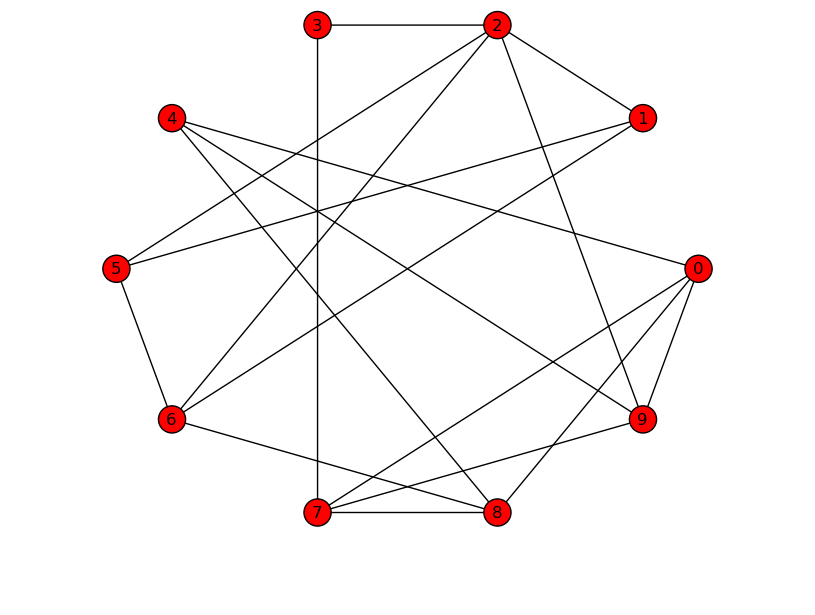
\includegraphics[scale=0.5]{imgs/binomial-10-04.png}
	  \end{center}
		\label{results:graph:binomial}
		\caption{Sample random binomial graph with $10$ nodes and a $40\%$ probability to create an edge between each pair of nodes.}
	\end{figure}
	}
	\defitem{Holme-Kim}{Also known as powerlaw cluster graphs\cite{holme2002growing}, the graph is constructed iteratively by attaching each new node to a number $t$ of already existing nodes using preferential attachment based on the degree of existing nodes. Also, after the addition of each edge, there is a probability $p$ that a triangle will be created by adding an additional edge. These graphs are controlled by two parameters: node count $n$ and density $p$; value $t$ is inferred as the product between $p$ and $n$.
	\begin{figure}
	  \begin{center}
	    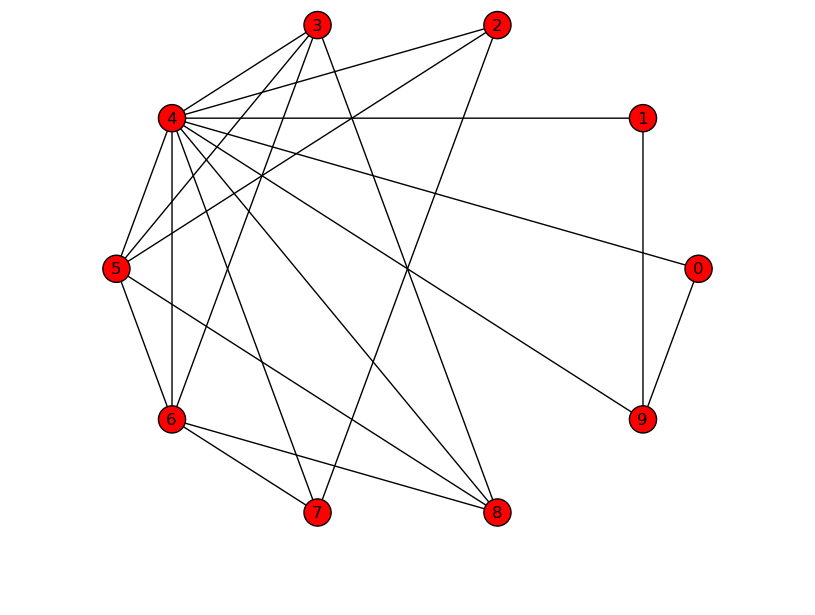
\includegraphics[scale=0.5]{imgs/hk-10-04.png}
	  \end{center}
		\label{results:graph:binomial}
		\caption{Sample random powerlaw cluster graph with $10$ nodes, note how certain nodes have a much higher degree than the others.}
	\end{figure}
	} 
\end{itemize}

Since both of the previous procedures generate unpartitioned graphs, they are partitioned after their generation by grouping nodes with consecutive indices in partitions of a certain size. For most instances we used a fixed partition size of $2$, although in some cases we used random sizes varying from $1$ to $4$.

These random graphs were generated using the \textit{NetworkX} python package\cite{networkx}, version $1.1$.